% $Id: SelectedCommands.tex,v 1.1 2008/01/31 18:04:17 dconway Exp $
\chapter{\label{chapter:SpecificCommands}Specific Command Details}
\chapauthor{Darrel J. Conway}{Thinking Systems, Inc.}

Chapter~\ref{chapter:Commands} provided an introduction and description of the GMAT command classes
and their usage when building a Mission Control Sequence.  In this chapter, the command
classes are described on a class by class level.

\section{\label{section:CommandClasses}Command Classes}

\begin{figure}[htb]
\begin{center}
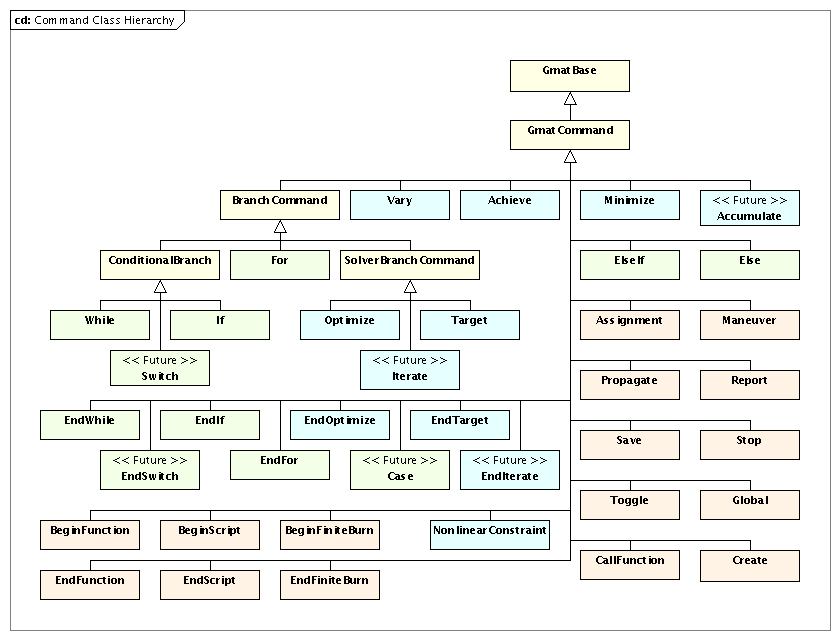
\includegraphics[420,320]{Images/CommandClassHierarchy.png}
\caption[GMAT Command Classes]{\label{figure:CommandClassDiagram}GMAT Command Classes.\\Classes
shown in yellow are base classes, green are control flow commands, blue are commands related to
Solvers, and orange are stand alone commands.}
\end{center}
\end{figure}

Figure~\ref{figure:CommandClassDiagram} shows the command classes incorporated into GMAT at this
writing.  The base class elements GmatCommand, BranchCommand, ConditionalBranch, and
SolverBranchCommand are described in Chapter~\ref{chapter:Commands}.  This chapter looks at the
details of the derived classes shown in the figure, providing implementation specifics for these
commands.  The following paragraphs review the role played by the command base classes and identify
pertinent utilities supplied by these bases that the derived classes use to implement their
capabilities.

\subsection{The GmatCommand Class}

Every entry in the mission control sequence is implemented as a class derived from GmatCommand.
This base class defines the interfaces used for the linked list structures that implement the
control sequence.  The \texttt{next} and \texttt{previous} members implement the links for the list
structure.

Commands are initialized in the Sandbox, as described in
Section~\ref{section:SandboxInitialization}.  They contain three data structures, set by the
Sandbox, that are used to set pointers correctly prior to execution.  These structures,
\texttt{objectMap}, \texttt{solarSys}, and \texttt{publisher}, are the structures managed by the
Sandbox to run a misison control sequence.  The \texttt{objectMap} and \texttt{solarSys} are the
local copies of the configured objects and space environment used when running the model, and need
to be accessed and used to set the pointers required in the commands to run in the Sandbox.  This
setup is performed in the command's Initialize() method.  The \texttt{publisher} member is a
pointer to the global GMAT Publisher, used to send data to the Subscriber subsystem.

Each GmatCommand implements the Execute() method defined in GmatCommand.  This method, along with
the internal supporting data structures and support methods, distinguish one command from another.
Execute() performs the actions built into the command, manipulating the configured objects to make
the model evolve in the Sandbox.

The GmatCommand class provides a generic implementation of the InterpretAction() method, used when
parsing lines of script.  Derived classes that need special handling for this parsing override
InterpretAction() to implement the parsing.  The GmatCommand base includes an instance of the
TextParser so that derived commands have the facilities provided for parsing.

\subsection{Branch Commands}

Nesting in the mission control sequence is implemented through the BranchCommand base class.  This
class, derived from GmatCommand, adds one or more branches to the main misison sequence.  The core
feature os the BranchCommands is the ability to execute these branches when conditions dictate that
the branch should execute.  This feature provides users with the ability to execute commands
conditionally, to loop over a set of commands, and to run routines that tune the mission to meet or
optimize selected goals.

\subsubsection{Conditional Branch Commands}

Some branch commands need the ability to evaluate conditions in order to determine if a branch
should be executed.  THe ConditionalBranch class provides the structures needed to identiofy and
evaluate these conditions.

\subsubsection{Solver Commands}

The Solver subsystem uses several commands designed to interoperate with the Solvers.  Because of
the close linkage between these commands and the corresponding solvers, the description for these
commands is given in Section~\ref{section:SolverCommandDescriptions}.  The commands defined in that
section are the branch commands Iterate/EndIterate, Target/EndTarget, and Optimize/EndOptimize, and
the GmatCommands Vary, Achieve, Minimize, NonlinearConstraint, Gradient, and TBD commands
associated with the scanners.

The nature of the problem encountered when running the Solvers requires that the sytates of many of
the objects defined in the Sandbox be stored at the start of the Solver execution, so that they can
be reset as the Solver iterates over the variables used to perform its tasks.  The
SolverBranchCommand class provides the data structures and methods needed to maintain these states
while the Solvers are performing their tasks.

\subsection{Functions}

\textit{To be filled in}

\section{Command Details}

\subsection{\label{section:Assignment}The Assignment Command}

Assignment commands implement the methods necessary for users to pass data into and between objects,
and to create copies of objects at specific points in the model, for use in the mission control
sequence.  Assignment commands are used to set one or more object properties while executing the
mission control sequence.  As can be see in Table~\ref{Table:AssignmentCommand}, the command has the
general form

\begin{equation}
\texttt{LHS}=\texttt{RHS}
\end{equation}

\noindent where the \texttt{LHS} entry is a single object or object property, and the \texttt{RHS}
entry is a number, object or object property, or equation.

%-----------------------------------------------------------------------
%-----------------------Begin Table Here--------------------------------
%----- (Comment the \clearpage code if the table doesn't break ----------
%------ across multiple pages or is the first in a section) ------------
%-----------------------------------------------------------------------
%\clearpage
\noindent
\tablecaption{Assignment Command}
\tablefirsthead{\hline\hline}\label{Table:AssignmentCommand}\index{\st{Assignment}}
\tablehead{\multicolumn{2}{c}{Table~\ref{Table:AssignmentCommand}: Assignment Command \ldots
continued}\\\\ \hline\hline}
\tabletail{\hline\hline}
\tablelasttail{\hline\hline}
\begin{supertabular*}{6.5 in}{@{}p{1.5 in}@{\extracolsep{\fill}}p{5.0 in}@{}}
    \multicolumn{2}{l}{}\\
    \multicolumn{2}{l}{Script Syntax: \st{GMAT Arg1 = Arg2;}}\\\\
    \hline\hline
    Command Description\\
    \hline
    %------- New Item
    \st{Arg1} & Default: N/A . Options:[Spacecraft Parameter, Array element, Variable,
    or any other single element user defined parameter]:
    %  Description
    The \st{Arg1} option allows the user to set \st{Arg1} to \st{Arg2}. Units: N/A.\\
    \st{Arg2} & Default: N/A . Options:[Spacecraft Parameter, Array element, Variable,
    any other single element user defined parameter, or a combination of the aforementioned
    parameters using math operators]:
    %  Description
    The \st{Arg2} option allows the user to define \st{Arg1}. Units: N/A.\\\\

    \hline\hline
    \multicolumn{2}{c}{Script Examples}\\
    \hline
    \multicolumn{2}{l}{\% Setting a variable to a number}\\
    \multicolumn{2}{l}{\st{GMAT testVar = 24;}}\\
    \multicolumn{2}{l}{\% Setting a variable to the value of a math statement}\\
    \multicolumn{2}{l}{\st{GMAT testVar = (testVar2 + 50)/2;}}\\\\

\end{supertabular*}\\


\subsection{\label{section:Propagate}The Propagate Command}

Propagation is controlled in the Mission Control Sequence using the Propagate command, which has
syntax described in Table~\ref{Table:PropagateCommand}.

%--------------------------------------------------------------------
%-----------------------Begin Table Here-----------------------------
%----- (Comment the \clearpage code if the table doesn't break ------
%------ across multiple pages or is the first in a section) ---------
%--------------------------------------------------------------------
%\clearpage
\noindent \tablecaption{Propagate Command}
\tablefirsthead{\hline\hline}\label{Table:PropagateCommand}
\tablehead{\multicolumn{2}{c}{Table ~\ref{Table:PropagateCommand}:
Propagate Command \ldots continued}\\\\ \hline\hline}
\tabletail{\hline\hline} \tablelasttail{\hline\hline}
\begin{supertabular*}{6.5 in}{@{}p{1.0 in}@{\extracolsep{\fill}}p{5.0 in}@{}}
    \multicolumn{2}{c}{ScriptSyntax}\\
    \hline\\
    \multicolumn{2}{l}
    {\st{Propagate Mode BackProp \emph{PropagatorName}(SatList1,\{StopCondList1\}) \ldots}}\\
    \multicolumn{2}{l}{\st{BackProp\emph{PropagatorName}(SatListN,\{StopCondListN\})}}\\\\

    \hline\hline
    Option & Option Description\\
    \hline
    %------- New Item
    \st{BackProp} & Default: None. Options: [ Backwards or None ]:
    The \st{BackProp} option allows the user to set the flag to enable or disable backwards propagation for all
    spacecraft in the the \st{SatListN} option.
    The Backward Propagation GUI check box field stores all the data in \st{BackProp}. A check indicates backward
    propagation is enabled and no check indicates forward propagation. In the script, \st{BackProp} can be the word
    Backwards for backward propagation or blank for forward propagation. Units: N/A.
    \index{\st{Backwards Propagation}}\\\\
    %------- New Item
    \st{Mode} & Default: None.  Options: [ Synchronized or None ]:
    The \st{Mode} option allows the user to set the propagation mode for the propagator that will affect all of the
    spacecraft added to the \st{SatListN} option. For example, if synchronized is selected, all spacecraft are
    propagated at the same step size. The Propagate Mode GUI field stores all the data in \st{Mode}. In the script,
    Mode is left blank for the None option and the text of the other options available is used for their respective
    modes. Units: N/A. \index{\st{Propagation Mode}}\\\\
    %------- New Item
    \emph{PropagatorName} & Default: DefaultProp. Options: [ Default propagator or any user-defined propagator ]:
    The \emph{PropagatorName} option allows the user to select a user defined propagator to use in spacecraft and/or
    formation propagation. The Propagator GUI field stores all the data in \emph{PropagatorName}. Units: N/A.\\\\
    %------- New Item
    \st{SatListN} & Default: DefaultSC. Options: [ Any existing spacecraft or
    formations, not being propagated by another propagator in the same Propagate event.  Multiple spacecraft must be
    expressed in a comma delimited list format. ]: The \st{SatListN} option allows the user to enter all the
    satellites and/or formations they want to propagate using the \emph{PropagatorName} propagator settings.
    The Spacecraft List GUI field stores all the data in \st{SatListN}. Units: N/A.\\\\
    %------- New Item
    \st{StopCondListN} /Parameter & Default: DefaultSC.ElapsedSecs =. Options: [ Any single element user accessible
    spacecraft parameter followed by an equal sign ]. The
    \st{StopCondListN} option allows the user to enter all the parameters used for the propagator stopping condition.
    See the \st{StopCondListN}/Condition Option/Field for additional details to the \st{StopCondListN} option.
    Units: N/A. \\\\
    %------- New Item
    \st{StopCondListN} /Condition & Default: 8640.0. Options: [ Real Number, Array element, Variable, spacecraft
    parameter, or any user defined parameter ].
    The \st{StopCondListN} option allows the user to enter the propagator stopping condition's value for the
    \st{StopCondListN} Parameter field. Units: Dependant on the condition selected. \\\\

    \hline\hline
    \multicolumn{2}{c}{Script Examples}\\
    \hline
    \multicolumn{2}{l}{\% Single spacecraft propagation with one stopping condition}\\
    \multicolumn{2}{l}{\% Syntax \#1}\\
    \multicolumn{2}{l}{\st{Propagate DefaultProp(DefaultSC, \{DefaultSC.ElapsedSecs = 8640.0\});}}\\\\

    \multicolumn{2}{l}{\% Single spacecraft propagation with one stopping condition}\\
    \multicolumn{2}{l}{\% Syntax \#2}\\
    \multicolumn{2}{l}{\st{Propagate DefaultProp(DefaultSC) \{DefaultSC.ElapsedSecs = 8640.0\};}}\\\\

    \multicolumn{2}{l}{\% Single spacecraft propagation by one integration step}\\
    \multicolumn{2}{l}{\st{Propagate DefaultProp(DefaultSC);}}\\\\

    \multicolumn{2}{l}{\% Multiple spacecraft propagation by one integration step}\\
    \multicolumn{2}{l}{\st{Propagate DefaultProp(Sat1, Sat2, Sat3);}}\\\\

    \multicolumn{2}{l}{\% Single formation propagation by one integration step}\\
    \multicolumn{2}{l}{\st{Propagate DefaultProp(DefaultFormation);}}\\\\

    \multicolumn{2}{l}{\% Single spacecraft backwards propagation by one integration step}\\
    \multicolumn{2}{l}{\st{Propagate Backwards DefaultProp(DefaultSC);}}\\\\

    \multicolumn{2}{l}{\% Two spacecraft synchronized propagation with one stopping condition}\\
    \multicolumn{2}{l}{\st{Propagate Synchronized DefaultProp(Sat1, Sat2, \{DefaultSC.ElapsedSecs = 8640.0\});}}\\\\

    \multicolumn{2}{l}{\% Multiple spacecraft propagation with multiple stopping conditions and propagation settings}\\
    \multicolumn{2}{l}{\% Syntax \#1}\\
    \multicolumn{2}{l}{\st{Propagate Prop1(Sat1,Sat2, \{Sat1.ElapsedSecs = 8640.0, Sat2.MA = 90\}) \ldots}}\\
    \multicolumn{2}{l}{\st{Prop2(Sat3, \{Sat3.TA = 0.0\});}}\\\\

    \multicolumn{2}{l}{\% Multiple spacecraft propagation with multiple stopping conditions and propagation settings}\\
    \multicolumn{2}{l}{\% Syntax \#2}\\
    \multicolumn{2}{l}{\st{Propagate Prop1(Sat1,Sat2) \{Sat1.ElapsedSecs = 8640.0, Sat2.MA = 90\}} \ldots}\\
    \multicolumn{2}{l}{\st{Prop2(Sat3) \{Sat3.TA = 0.0\};}}\\
\end{supertabular*}\\


\noindent Each Propagate command identifies one or more PropSetup\footnote{The object used in this
role in GMAT is an instance of the PropSetup class.  On the GUI and in GMAT scripting, the keyword
used for PropSetup instances is ``Propagator.''  In this document I'll use the class name,
PropSetup, when referring to these objects.}, consisting of an integrator and forcemodel defined to
work together.  Each PropSetup identifies one or more SpaceObject that it is responsible for
advancing through time.  This propagation framework allows users to model the motion of one or more
SpaceObjects using different propagation modes, and to advance the SpaceObjects to specific points
on the SpaceObject's trajectories.

\subsubsection{Propagation Modes}

The Propagate command provides several different modes of propagation based on the settings passed
into the command.  These modes are described in the following list:

\begin{itemize}
\item \textbf{Unsynchronized Propagation}  Unsynchronized propagation is performed by executing the
PropSetups assigned to a Propagate command independently, allowing each PropSetup to find its
optimal step without regard for other PropSetups assigned to the command.
\item \textbf{Synchronized Propagation}  Synchronized propagation steps the first PropSetup
assigned to the command using its optimal step, and then advances the remaining PropSetups by the
same interval, so that the epochs for all of the PropSetups remain synchronized during integration.
\item \textbf{Backwards Propagation}  GMAT usually integrates SpaceObjects so that the epoch of the
SpaceObject increases.  Integration can also be performed so that the epoch decreases, modeling
motion backwards in time.
\item \textbf{Propagation to Specific Events}  Propagation can be performed
in GMAT until specific events occur along a SpaceObject's trajectory.  When the one of these
specified events occurs, the Propagate command detects that a condition requiring termination of
propagation has occurred, finds the time step required to reach the epoch for that termination, and
calls the PropSetups to propagate the SpaceObjects for that period.
\item \textbf{Single Step Propagation}  When no specific events are specified as stopping
conditions, the Propagate command takes a single propagation step and exits.
\end{itemize}

\subsubsection{The Propagation Algorithm}

\begin{figure}[htb]
\begin{center}
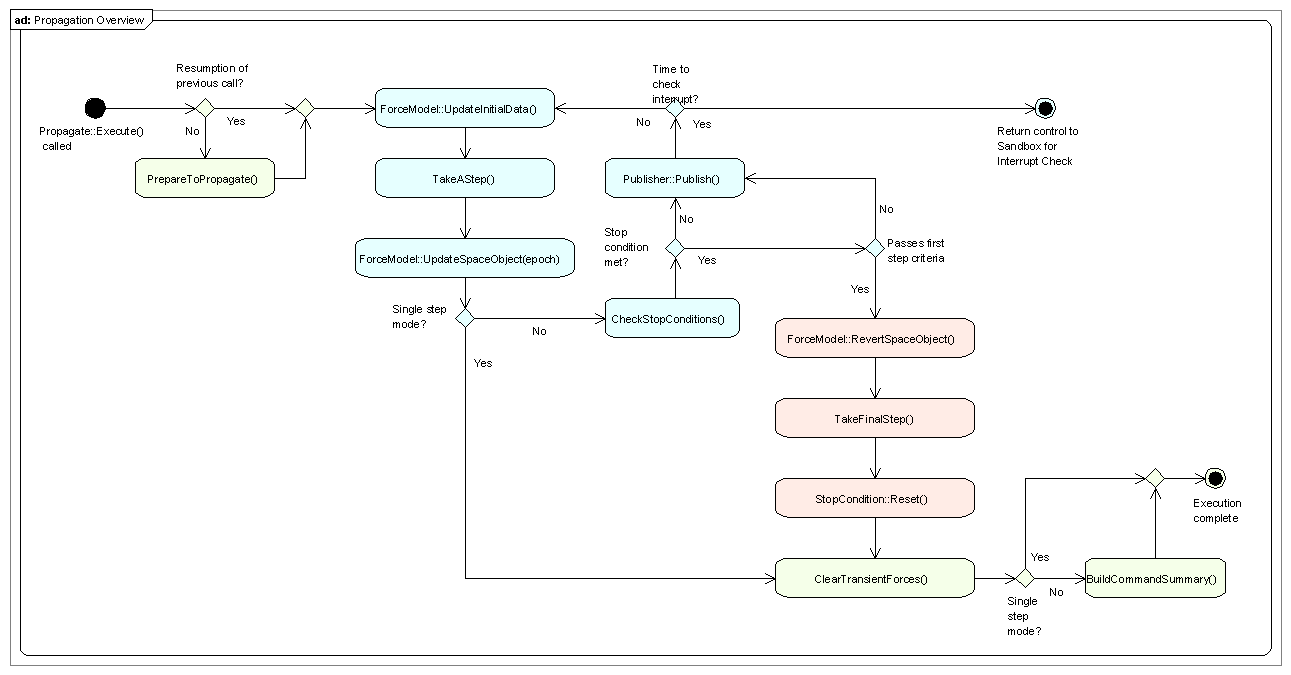
\includegraphics[445,233]{Images/PropagationOverview.png}
\begin{quote}
\caption[Executing the Propagate Command]{\label{figure:PropagateExecute}Executing the
Propagate Command\\The core propagation code is shown in blue.  Steps taken during startup and
shutdown are colored green.  Steps used when stopping propagation at specific events are shown in
red; additional details for the stopping condition algorithm are described below and shown in
Figure~\ref{figure:StopAlgorithm}.}
\end{quote}
\end{center}
\end{figure}

Figure~\ref{figure:PropagateExecute} shows the basic process implemented in the Propagate command.
Propagation usually consumes the bulk of the time required to run a mission in GMAT.  Because of
this feature, the Propagate command was written to support execution across several steps in the
Sandbox, so that the Sandbox can poll for user interruption during propagation.  There are several
initialization steps required at the start of propagation that should not be performed when
reentering the command from a polling check in the Sandbox.  These steps are performed in the
PrepareToPropagate() method identified in the figure.

Once the Propagate command is ready to perform propagation, the force models used in propagation are
initialized to the start of the step about to be taken, and then the PropSetups take a single
integration step.  The resulting integrated states are passed into the relevant SpaceObjects through
calls to the ForceModel's UpdateSpaceObject methods.

The next action depends on the propagation stopping mode: if the Propagate command is operating in
single step mode, propagation is complete and control exits the propagation loop.  Otherwise, the
stopping conditions are evaluated and compared to the desired stopping events.  If no stopping
conditions have been passed or met, the integrated state data is passed to GMAT's Publisher for
distribution.  The command then determines if an interrupt check is required; if so, control is
returned to the Sandbox for the check, otherwise, the propagation loop resumes with an update to the
ForceModel.

If a stopping condition was triggered, it is first tested to ensure that the triggered stopping
condition is not an artifact of a previous propagation execution.  This test is only performed
during the first propagation step of a new execution.  If the stopping condition passes this
validation, control leaves the main propagation loop and enters the control logic implemented to
terminate propagation at a specific stopping event, as described in the next section.

Once the propagation has been terminated, any transient forces set during propagation are cleared
from the force models, command summary data is set when running with stopping conditions, and
execution is completed.

\subsubsection{The Stopping Algorithm}

\begin{figure}[htb]
\begin{center}
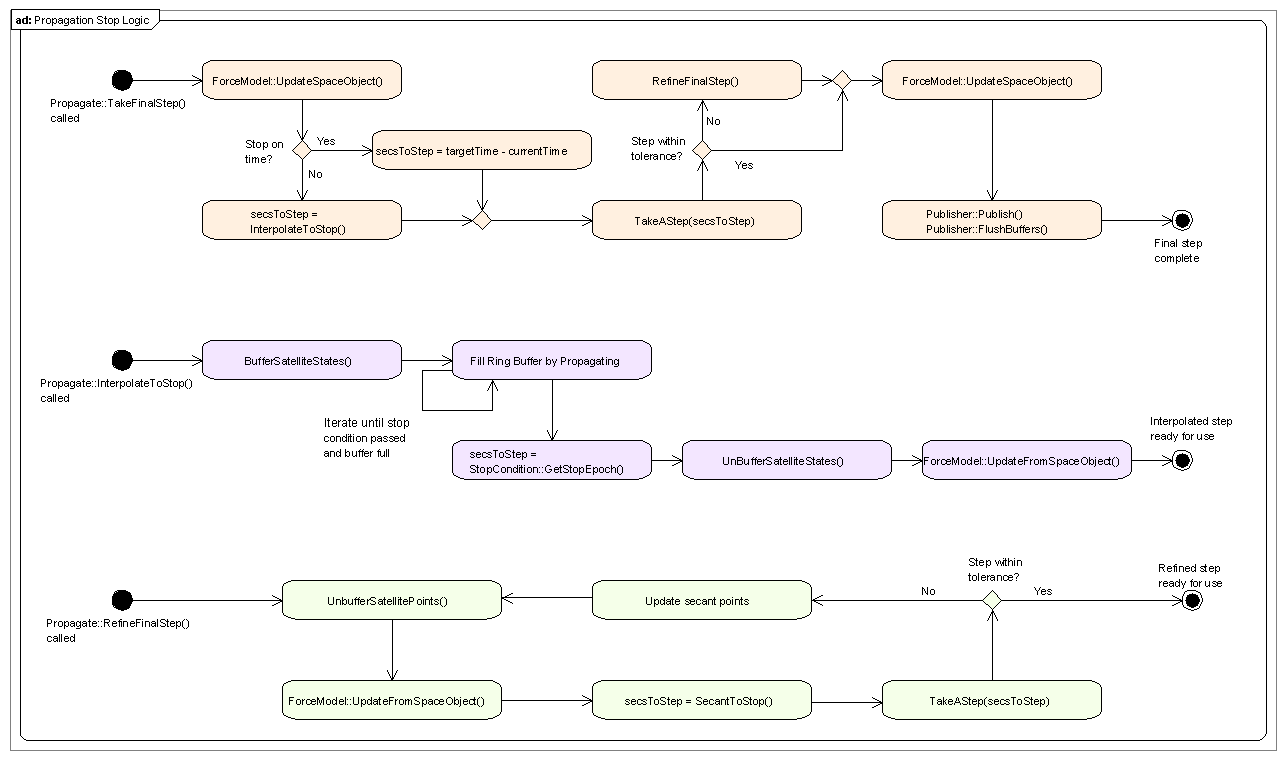
\includegraphics[445,284]{Images/PropagationStopLogic.png}
\begin{quote}
\caption[Algorithm Used to Stop Propagation]{\label{figure:StopAlgorithm}Algorithm Used to Stop
Propagation\\The core algorithm is shown in orange, in the sequence at the top of the figure.  The
initial estimate of the time step needed to reach the stop epoch is performed using a cubic spline
algorithm; this sequence is shown in purple in the center of the diagram.  If further refinements
are needed, they are made using a secant algorithm, shown in the lower, green portion of the
figure.}
\end{quote}
\end{center}
\end{figure}

Propagation performed to reach specific events is terminated at points within a fixed tolerance of
those events.  The algorithm employed to take this final step is shown in
Figure~\ref{figure:StopAlgorithm}.  Propagation used time as the independent parameter to evolve
the states of the propagated SpaceObjects, so the stopping condition problem can be reduced to
finding the time step that moves the SpaceObjects from the propagated state immediately prior to
the desired event up to that event.  The steps shown in the figure are used to find that time
step, and to advance the SpaceObject states by that amount.

\paragraph{Stopping Condition Evaluation.}  The top portion of the figure shows the basic stopping
condition evaluation procedure in the command.  First the force model is prepared for a propagation
step.  If the stopping condition is a time based condition, the time step is estimated by
subtracting the desired time from the current time.  Stopping conditions that are not time based are
estimated using a cubic spline algorithm, designed to avoid knots at the second and fourth points
used when building the splines (see the description of the not-a-knot cubic spline in
\cite{mathSpec}).  The steps performed when running the cubic spline are shown in the central
portion of the figure and described below.

After the time step needed to reach the desired event has been estimated, the SpaceObjects are
propagated using that time step.  The resulting values for the stopping parameters are calculated
and compared to the desired stop values.  If the result is not within the stopping tolerance for
the propagation, a further refinement is made to the time step estimate using a secant based
implementation of Newton's method, described below and illustrated in the bottom portion of the
figure.

Once the final propagation step has been performed to acceptable tolerance, the resulting
propagated states are applied to the SpaceObjects.  The Publisher is passed the new state data and
instructed to empty its data buffers.  This completes the stopping algorithm.

\paragraph{Cubic Spline Details.}  The heart of the stop time estimation for events that are not
time based is the not-a-knot cubic spline algorithm.  The problem solved using this algorithm
inverts the roles of the independent variable -- the propagation time -- and the dependent variable
-- the parameter that is advancing to reach some specific event -- so that the desired time step
can be generated based on the desired event value.  Since we already know the time step that
advances the SpaceObject states from one side of the desired event to the other, we have the time
steps that bracket the stop time, and we need only refine this time using the spline interpolator.

The spline algorithm requires five pairs of data points to estimate this time.  These data points
are generating by propagating the SpaceObjects across the time interval that brackets the stop
event in four equally spaced steps, evaluating the stop parameter after each step.  These values
and associated times, along with the parameter value and time at the start of the process, are used
by the spline to estimate the time step needed to reach the target event.  The implementation
details, as shown in the figure, are described in the following paragraphs.

Before performing the necessary propagations, the SpaceObject states at the start of the procedure
are buffered so that they can be restored later.  The SpaceObjects are then propagated for a
minimum of four steps, checking to ensure that the stop event is actually crossed.  If the desired
event is not crossed, additional propagation steps -- up to a maximum of four additional steps --
are allowed in order to continue searching for the condition required for stopping.  If the event
is still not encountered, and exception is thrown and execution terminates.

Once the spline buffer has been filled with values that bracket the stop event, the spline algorithm
is called to get the time step that is estimated to produce target value.  This time step is stored,
the buffered states are reset on the SpaceObjects, and the force model is reset in proparation for a
final propagation step.  This completes the spline interpolation portion of the stopping condition
evaluation.

\paragraph{Additional Refinements using a Secant Solver.}  For most stopping reqirements encountered
in GMAT, the not-a-knot cubic spline solution described above is sufficiently accurate.  However,
there are cases in wich the propagation needs further refinement to meet mission requirements.  In
those cases, the cubic spline solution is refined using a secant based root finder.  The resulting
algorithm, shown in the bottom portion of Figure~\ref{figure:StopAlgorithm}, is described in the
following paragraphs.

The data in the force model at this point in the process is the propagated state data generated
using the time step obtained from the cubic spline.  Before proceding, these data are replaced with
the state data at the start of the final step.

The next estimate, $t_2$, for the desired time step is made using the target parameter value,
$v_T$, the calculated parameter value, $v_0$ at the epoch $t_0$ of the initial state and the value,
$v_1$, obtained after the spline step, $t_1$, was applied using the formula

\begin{equation}
t_2 = v_T \frac{t_1-t_0}{v_1-v_0}.
\end{equation}

\noindent This formula is evaluated in the SecantToStop method.  The resulting time step is then
applied to the SpaceObjects.  If the resulting parameter value is withing acceptable tolerance, the
refinement algorithm terminates.  If not, the results from this new step are stored, the state data
and force model are reset, and a new time step is calculated using the equation

\begin{equation}
t_{n+1} = v_T \frac{t_n-t_{n-1}}{v_n-v_{n-1}}.
\end{equation}

\noindent This process repeats until either an integration step is taken that meets the propagator
tolerance requirements, or an unacceptable number of attempts have been made and failed.  The
Propagate command will make 50 such attempts before raising an exception and termminating execution.

\subsubsection{The Startup and Shutdown Routines}

There are several steps that need to be applied before and after propagation to ensuree htat
propagation uses and releases data that depends on the current state of the mission control
sequence.  The following paragraphs destribe these steps.

\paragraph{During startup}, the Propagate command updates the object pointers and data structures to
match the current state of the objects in the mission.  \textit{More to come here.}

\paragraph{Upon completion} of propagation, the Propagate command resets its internal flags
indicating that the command is ready to be called at a new point in the mission and clears any
transient forces that have been set for the current propagation.  If the command is not running in
single step mode, the states of the SpaceObjects are accessed and stored in the command summary
buffers for display on user request.  (This operation is moderately expensive computationally, so it
is not performed in single step mode.)  This completes execution of the Propagate command.

\subsubsection{Propagate Command Attributes and Methods}

The class design for the Propagate command is shown in Figure~\ref{figure:PropagateCommand}.

\begin{figure}[htb]
\begin{center}
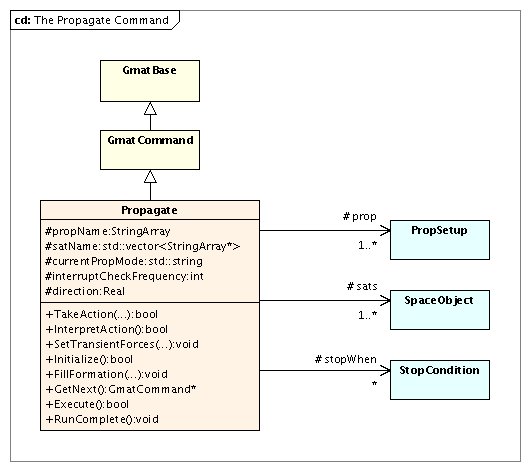
\includegraphics[265,238]{Images/ThePropagateCommand.png}
\caption{\label{figure:PropagateCommand}Propagate Command Details}
\end{center}
\end{figure}

\subparagraph{\textit{Class Attributes}}

Each Propagate command instance implements the following data elements:

\begin{itemize}
\item \textbf{StringArray propName}:  List of the PropSetups used in this command.
\item \textbf{std::vector<StringArray*> satName}:  A vector of lists of SpaceObjects.  There is a
1:1 correspondence between the propName members and the satName StringArrays.  In addition, each of
these StringArrays must have at least one member, and that member must be the name of a SpaceObject.
\item \textbf{std::string currentPropMode}:  The propagation mode setting for the PropSetups.  This
string tracks whether the propagation is synchronized or not\footnote{GMAT currently supports two
propagation modes, synchronized -- specified by the keyword ``Synchronized'', and unsynchronized,
the default setting.  Backwards propagation is treated separately, though the ``BackProp'' keyword
is parsed as a propagation mode.}.
\item \textbf{Real direction}: The propagation direction: 1.0 to propagate forwards in time, -1.0
to propagate backwards.
\item \textbf{int interruptCheckFrequency}:  The number of steps the PropSetup will take before
returning control to the Sandbox.  This setting is used to allow the Sandbox to poll for interrupts
from the user, as described in Section~\ref{section:SandboxInterruptPolling}.
\item \textbf{std::vector<PropSetup *> prop}:  The PropSetups used in this instance.
\item \textbf{std::vector<SpaceObject *> sats}:  The SpaceObjects propagated by the PropSetups.
\item \textbf{std::vector<StopCondition *> stopWhen}:  The stopping conditions used to determine
when propagation should terminate.  If no stopping conditions are specified, the PropSetups fire
the mminimum number of times allowed -- one time in unsynchronized mode, and just enough times to
meet the synchronization constraint in synchronized mode.
\end{itemize}

\subparagraph{\textit{Methods}}

The public methods implemented in the Propagate command are itemized below:

\begin{itemize}
\item \textbf{bool TakeAction(const std::string \&action, const std::string \&actionData)}:
Performs actions specific to propagation.  The Propagate command defines three actions:
\begin{itemize}
\item \textit{Clear}: Clears the arrays of reference objects used by the instance.  Clearing can
occur for two distinct types of objects:
\begin{itemize}
\item \underline{Propagator}: Clears the lists of PropSetups, propagated SpaceObjects, and the
associated StringArrays.
\item \underline{StopCondition}:  Clears the lists of stopping conditions, SpaceObjects used for
stoppign, and any associated StringArrays.
\end{itemize}
\item \textit{SetStopSpacecraft}: Adds a named SpaceObject to the list of SpaceObjects used for
stopping.
\item \textit{ResetLoopData}: Resets the PropSetups to their startup values so that Solvers obtain
consistent results when iterating to a solution.
\end{itemize}
\item \textbf{void FillFormation(SpaceObject* so, StringArray owners, StringArray elements)}:  Fills
in the components of a formation recursively.
\item \textbf{GmatCommand* GetNext()}: Returns the next command that should be executed.  Propagate
overrides the implementation provided by GmatCommand so that interrupt polling can occur without
abnormally terminating propagation.
\item \textbf{bool InterpretAction()}:  The parser for the Propagate command, overridden from the
default implementation to handle all of the variations Propagate supports.
\item \textbf{void SetTransientForces(std::vector<PhysicalModel*> *tf)}:  Tells the Propagate
command about the current list of transient forces, so taht the command can incorporate active
transient forces into the force model in the PropSetups.
\item \textbf{bool Initialize()}:  Performs initialization in the Sandbox prior to execution of the
command.
\item \textbf{bool Execute()}:  Performs the propagation.
\item \textbf{void RunComplete()}:  Cleans up the command structures after completion of
propagation.
\end{itemize}


\subsection{The Create Command}

\subsection{The Target Command}

\subsection{The Optimize Command}
